\chapter{Estudo de caso}
\label{cap:estudodecaso}

Este capítulo apresentará a estrutura da empresa que será objetivo de estudo neste trabalho. Esta é uma empresa que fornece serviços de 
hospedagens e também está associada a um provedor de Internet\footnote{É importante salientar que esse provedor utiliza a maior parte dos 
serviços da empresa, pois possui maior número de clientes.}. A empresa possui grande parte de seus clientes localizados na serra do 
Rio Grande do Sul, sendo que atualmente essa empresa possui aproximadamente 9000 clientes. A sede da empresa está localizada na cidade de 
Garibaldi, além disso possui quatro filiais no estado, atendendo aproximadamente xx?? cidades.

A empresa oferece serviços pela internet aos seus clientes, sendo eles: hospedagens de sites, banco de dados, \textit{e-mail}, sistemas de gestão, 
\textit{e-mail marketing}, \textit{backup}, \textit{máquinas virtuais}, autenticação via \ac{ADSL}, rádio \textit{online} e telefonia.
Além disso, o provedor associado fornece aos seus clientes acesso à internet via rádio e acesso à internet por meio de fibra óptica.
A maioria dos serviços são fornecidos por meio de \textit{softwares} de código aberto.

Atualmente a empresa possui redundância de refrigeração e de energia, como pode ser observado na Figura \ref{fig:insteletrica}. 
A redundância de refrigeração é composta por dois ares-condicionados (identificar na figura ??). 
A redundância de energia é feita através de três \textit{nobreaks}, sendo que dois deles (identificar na fig ??) são utilizados para alimentação 
dos servidores e outros equipamentos como por exemplo roteadores, de forma que caso um falhe o outro alimente todos os equipamentos. O terceiro 
\textit{nobreak} (identificar na fig ??) é utilizado para alimentar os computadores dos funcionários de dois setores. 
Além disso, dois geradores (identificar nag fig ??) suprem a necessidade de consumo de energia elétrica do ambiente.
Na imagem também pode-se observar a entrada de energia, com três fases (RGE fase 1, RGE fase 2 e RGE fase 3). Ligado aos \textit{nobreaks} estão 
ligados seis \textit{totens} (são torres que possuem tomadas para plugar os equipamentos). E por fim os \textit{racks} onde ficam os servidores
e o restante dos equipamentos.

\begin{figure}[h!]
 \centering
 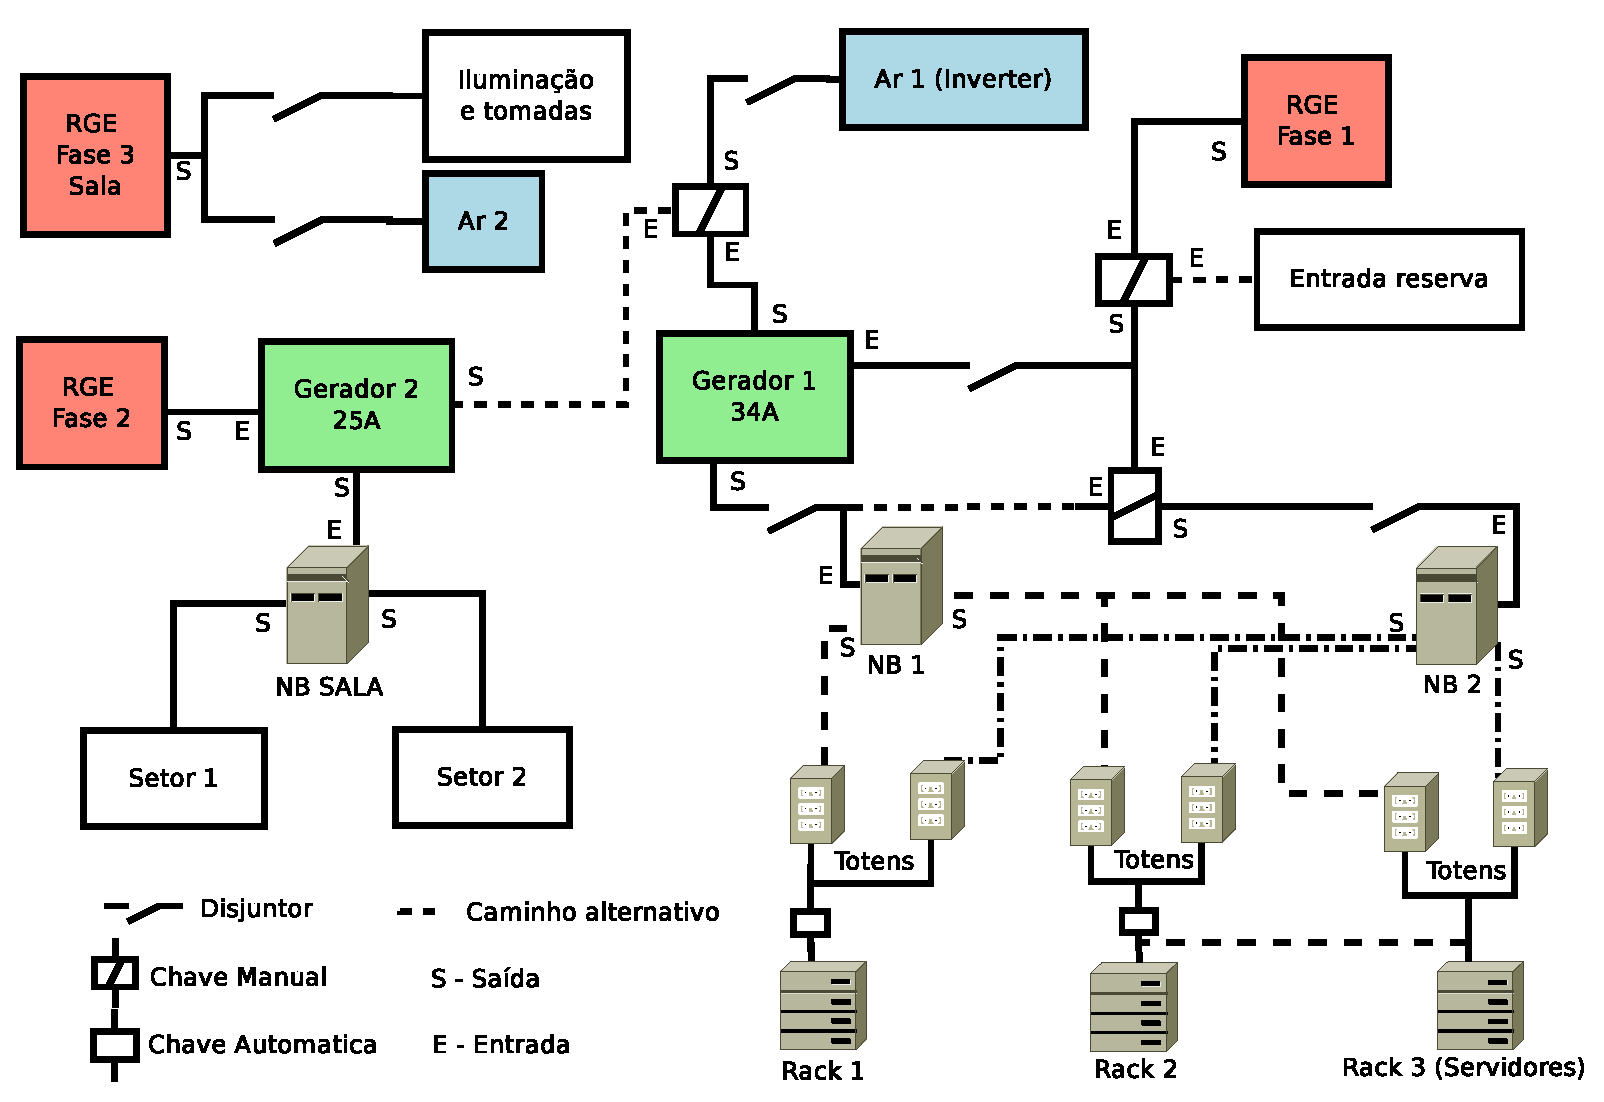
\includegraphics[width=380px]{img/insteletrica.eps}
 \caption{Diagrama de instalação elétrica.}
 \label{fig:insteletrica}
\end{figure}

Nas próximas seções será feita uma descrição da estrutura da empresa. Na Seção \ref{section:ambiente} será descrito o ambiente físico dos 
servidores, com suas estruturas e suas configurações. Na Seção \ref{section:servsemvirt} será descrito os servidores que possuem os seus
serviços instalados diretamente sobre o sistema operacional do servidor, ou seja, sem virtualização.
Na Seção \ref{section:servvirt} será descrito a estrutura de virtualização e todos os serviços fornecidos pelos servidores. 
E na Seção \ref{section:servcrit} será feito a seleção dos serviços críticos através de critérios definidos.

\section{Ambiente físico}
\label{section:ambiente}

A estrutura atual da empresa é composta por quatorze servidores físicos. 
A configuração de \textit{hardware} desses servidores pode ser encontrada na Tabela \ref{tab:servfisicos}, onde tem-se o nome do servidor, 
o modelo, a configuração dos processadores, quantidade de memória, número de discos e a capacidade unitária de cada disco.

\begin{table}[h!]
\caption{Configuração dos servidores físicos.}
\label{tab:servfisicos}
\begin{center}
\def\arraystretch{1}
\setlength{\tabcolsep}{0.15cm}
\begin{tabular}{|l|l|p{5.1cm}|l|p{2.1cm}|}\hline
Servidor & Modelo & Processador & Memória & Disco\\\hline
Bello & & 1 x Intel Core 2 Duo E6750 2.66 GHz & 2 GB DDR2 & 5,5 TB SATA\\\hline
Cacti & Dell PowerEdge 2950 & 2 x Intel Xeon E5310 1.60 GHz & 12 GB DDR2 & 2 x 73 GB SAS\\\hline
Dati & Dell PowerEdge 1850 & 2 x Intel Xeon 3.20 GHz & 4 GB DDR2 & 2 x 146 GB SCSI\\\hline
Monit & & 1 x Intel Core 2 Quad Q9550 2.83 GHz & 4 GB DDR2 & 120 GB SSD\\\hline
Nino & & 1 x Intel Core 2 Duo E4500 2.20 GHz & 4 GB DDR2 & 500 GB SATA\\\hline
Sfrunhon & & 1 x Intel Xeon X3330 2.66 GHz & 8 GB DDR2 & 750 GB SATA\\\hline
Vigilante & & 1 x Intel Pentium Dual E2180 2.00 GHz & 4 GB DDR2 & 2,5 TB SATA\\\hline
Brina & Dell PowerEdge 2950 & 2 x Intel Xeon E5410 2.33 GHz & 24 GB DDR2 & 6 x 300 GB SAS\\\hline
Fulmine & IBM System x3650 M4 & 1 x Intel Xeon E5-2650 2.00 GHz & 32 GB DDR3 & 6 x 2 TB SATA\\\hline
Piova & Dell PowerEdge R410 & 2 x Intel Xeon E5530 2.40 GHz & 32 GB DDR3 & 4 x 500G SATA\\\hline
Raggio & HP ProLiant DL360 G7 & 2 x  Intel Xeon E5630 2.53 GHz & 32 GB DDR3 & 4 x 300 GB SAS\\\hline
Tempesta & Dell PowerEdge R620 & 2 x Intel Xeon E5-2620 2.00 GHz & 32 GB DDR3 & 5 x 1 TB SATA 3 x 1,2 TB SAS\\\hline
Tuono & HP ProLiant DL380 G7 & 2 x Intel Xeon E5649 2.53 GHz & 32 GB DDR3 & 6 x 300 GB SAS 2 x 146 GB SAS\\\hline
Venti & Dell PowerEdge R210 II & 1 x Intel Xeon E3-1220 3.10 GHz & 16 GB DDR3 & 2 x 3 TB SATA\\\hline
\end{tabular}
\end{center}
\end{table}

Todos os servidores estão ligados ao \textit{switch}, que provê aos servidores acesso à internet através de um roteador. Para os servidores 
mais importantes são utilizados dois cabos de rede que estão ligados a um \textit{switch} \textit{gigabit}, assim possibilitando
a configuração de \textit{link aggregation} que permite configurar mais de uma interface de rede física em uma interface agregada, com isso 
pode-se dobrar a capacidade de tráfego de dados. 
O diagrama da Figura \ref{fig:servfisicos} demonstra uma visão geral da estrutura física dos servidores da empresa. 

\begin{figure}[h!]
 \centering
 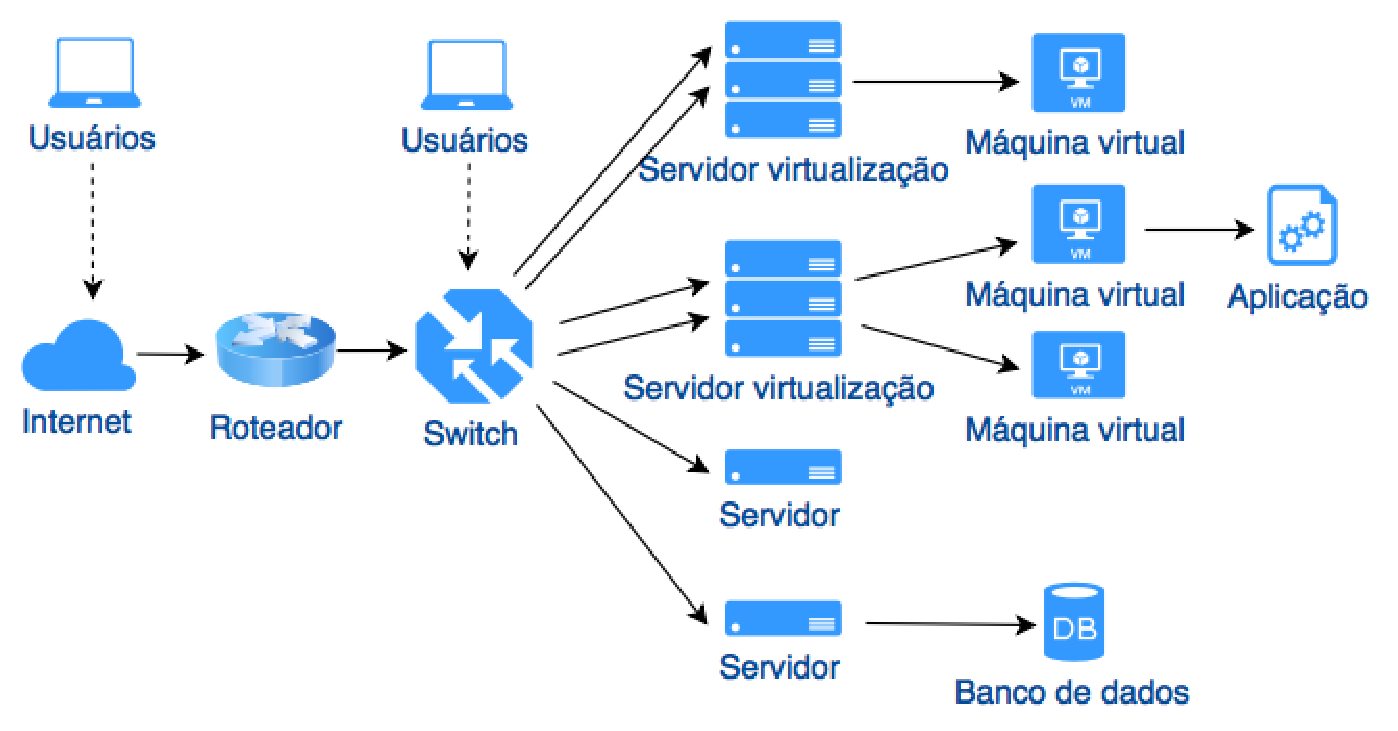
\includegraphics[width=380px]{img/servfisicos.eps}
 \caption{Modelo de estrutura física.}
 \label{fig:servfisicos}
\end{figure}

A Figura \ref{fig:servrack} demonstra, através de uma foto, todos os servidores, inclusive o \textit{switch}, montados em um \textit{rack}.

\begin{figure}[h!]
 \centering
 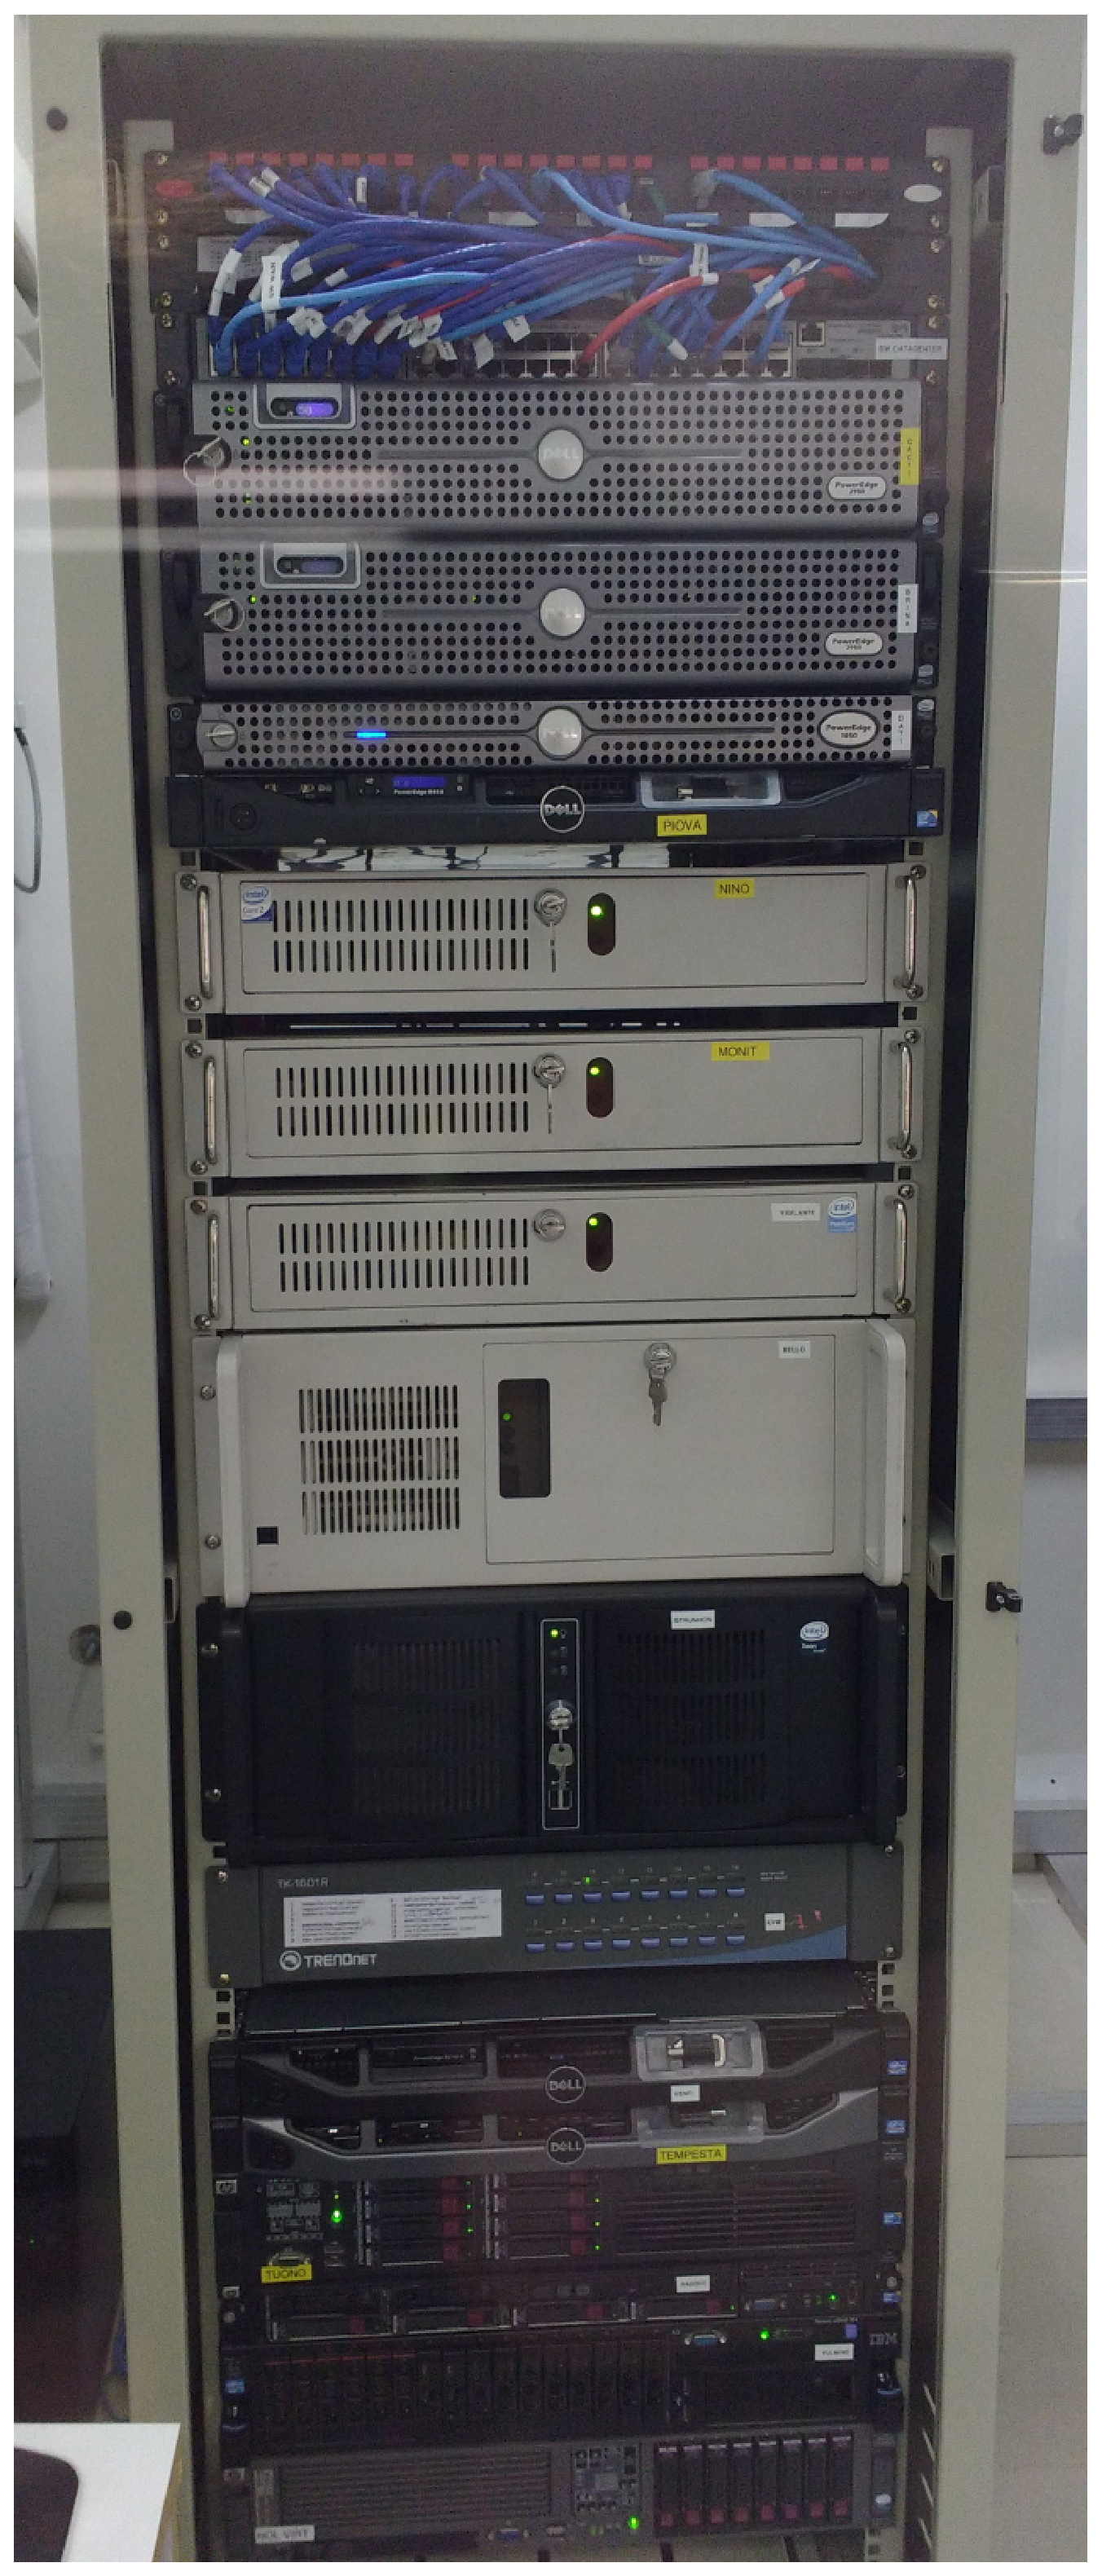
\includegraphics[width=120px]{img/servrack.eps}
 \caption{Imagem do \textit{rack} e dos servidores.}
 \label{fig:servrack}
\end{figure}

\section{Servidores sem virtualização}
\label{section:servsemvirt}

Atualmente existem sete servidores que possuem serviços onde executam sobre o sistema operacional nativo, ou seja, sem virtualização. 
Eles são os sete primeiros servidores da Tabela \ref{tab:servfisicos}, e são listados a seguir:
\begin{itemize}
 \item Bello: esse servidor possui o sistema operacional \textit{Ubuntu 14.04 \ac{LTS}} \cite{ubuntu}. Sua função é armazenar dados de 
 \textit{backup}, para isso ele possui a ferramenta \textit{Bacula Storage 5.2.6} \cite{bacula} instalado, que o possibilita fazer esse 
 armazenamento. Sendo que a ferramenta que é responsável por fazer o \textit{backup} está instalada em um outro servidor que será detalhado na 
 Seção \ref{section:serv_venti};
 
 \item Cacti: um dos servidores de monitoramento da rede do provedor. Esse utiliza a distribuição \textit{CentOS 6.6} \cite{centos} e executa a 
 aplicação \textit{Cacti 0.8.8b} \cite{cacti}, que é uma ferramenta de código aberto desenvolvida para monitorar qualquer equipamento de rede que 
 suporte o protocolo \ac{SNMP}. Ela monitora atualmente a maior parte da rede \textit{core} e a rede \textit{backbone} tanto dos clientes de 
 internet via rádio, como de fibra óptica;
 
 \item Dati: é o servidor de banco de dados principal. Esse possui o sistema operacional \textit{Ubuntu 14.04 \ac{LTS}} \cite{ubuntu}. 
 O serviço que executa sobre esse servidor é um sistema gerenciador de banco de dados \textit{MySQL 5.5.49} \cite{mysql}, que armazena os dados 
 das aplicações de \textit{ZoneMinder} \cite{zoneminder} (servidor de câmeras) e \textit{Icewarp Server} (servidor de e-mail), que serão 
 detalhados posteriormente;
 
 \item Monit: esse servidor faz o monitoramento dos demais servidores. Ele possui o sistema operacional \textit{Ubuntu 12.04 \ac{LTS}} 
 \cite{ubuntu}, executando as aplicações \textit{Nagios 3.2.3} \cite{nagios} e \textit{Munin 1.4.6} \cite{munin}, ambos \textit{softwares} livres. 
 O \textit{Nagios} monitora o \textit{hardware} e os serviços que estão executando em cada servidor. Para alguns serviços é utilizado um cliente 
 \textit{Nagios}. O segundo, \textit{Munin}, é responsável por gerar gráficos de monitoramento. Com ele pode-se criar, por exemplo, gráficos 
 com a utilização: do processador, memória, disco, temperatura e velocidade dos \textit{fans};
 
 \item Nino: esse é o servidor utilizado pelo setor de desenvolvimento de \textit{software}. Suas aplicações executam sobre o sistema operacional 
 \textit{Ubuntu 14.04 \ac{LTS}} \cite{ubuntu}, sendo que serviços fornecidos pelo servidor são servidor \textit{web} (\textit{Apache 2.4.7} 
 \cite{apache} e \textit{\ac{PHP} 5.5.9} \cite{php}), sistema gerenciador de banco de dados (\textit{MySQL 5.5.49} \cite{mysql} e 
 \textit{PostgreSQL 9.3.13} \cite{postgres}), compartilhamento de arquivos (\textit{Samba 4.3.9} \cite{samba}), controle de versões de 
 \textit{software} (\textit{\ac{SVN} 1.8.8} \cite{svn}), gerenciador de \textit{bugs} (\textit{Trac 1.0.1} \cite{trac}) e mensagens instantâneas 
 (\textit{Ejabberd 2.1.11} \cite{ejabberd});
 
 \item Sfrunhon: outro servidor de monitoramento da rede do provedor. Esse utiliza a distribuição \textit{CentOS 6.3} \cite{centos} e executa a 
 aplicação \textit{Cacti 0.8.8a} \cite{cacti}. Esse servidor monitora atualmente o tráfego dos clientes, tanto de internet via rádio, como de 
 fibra óptica;
 
 \item Vigilante: esse servidor é responsável por capturar e armazenar \textit{streaming} de vídeo das câmeras do provedor. Ele possui o sistema 
 operacional \textit{Ubuntu 14.04 \ac{LTS}} \cite{ubuntu}, e executa a aplicação \textit{ZoneMinder 1.29} \cite{zoneminder}, que é o 
 \textit{software} responsável pela captura e armazenamento das as imagens das câmeras do provedor.
\end{itemize}

\section{Servidores com virtualização}
\label{section:servvirt}

Os servidores de virtualização possuem suas respectivas \ac{VM}s, que executam aplicações. Para virtualização utiliza-se o hipervisor 
\ac{KVM} e a ferramenta \textit{QEmu}, sendo que ambos são projetos de \textit{software} livre. Procurou-se manter um ambiente homogêneo 
com o objetivo de facilitar a manutenção, para isso utilizou-se o mesmo hipervisor e o mesmo sistema operacional para os servidores hospedeiros. 
Esse sistema operacional é o sistema de código aberto \textit{Ubuntu 14.04 \ac{LTS}} \cite{ubuntu}.
Além disso, esses servidores possuem redundância de \textit{hardware}, com fonte de alimentação e discos configurados através de um \ac{RAID}. 
Em seridores com mais de dois discos geralmente é utilizado \ac{RAID} 5. Já em servidores que possuem apenas dois discos é utilizado \ac{RAID} 1 
(espelhamento de discos). O ambiente também possui uma redundância do cabeamento, como visto anteriormente.

A empresa fornece serviços diversos, desde hospedagens de sites até \ac{DNS} recursivo para o provedor de internet. Atualmente sete servidores 
são utilizados para virtualizar sistemas, que são os últimos sete servidores da Tabela \ref{tab:servfisicos}, sendo que existem quarenta e seis 
\ac{VM}s distribuídas entre os sete servidores de virtualização. A seguir será descrito esses servidores e suas respectivas máquinas virtuais.

O servidor Brina possui X?? \ac{VM}s, sendo que na Figura \ref{fig:serv_brina} está detalhado o servidor de virtualização, com suas máquinas 
virtuais e os serviços fornecidos. Esses serviços são listados a seguir:
\begin{itemize}
 \item \textit{Speedauth}: sua configuração é 2 \textit{cores} para processamento, 1,5 GB de memória e 8 GB de disco. O sistema operacional é o 
 \textit{Ubuntu 14.04 \ac{LTS}} \cite{ubuntu}. Esse é o servidor que fornece o serviço de autenticação \ac{PPPoE} para maior parte dos clientes do provedor 
 utilizando \textit{Radius} (\textit{Freeradius 2.1.12});
\end{itemize}

\begin{figure}[h!]
 \centering
 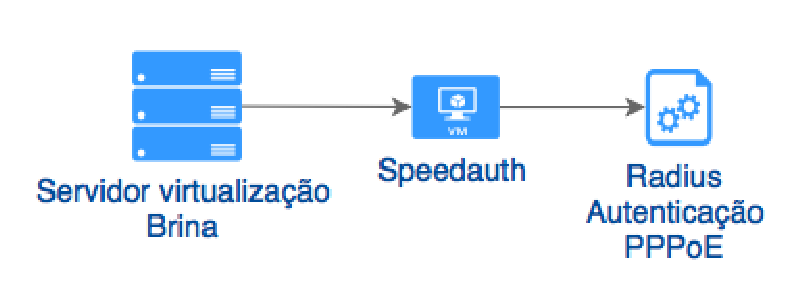
\includegraphics[width=250px]{img/serv_brina.eps}
 \caption{Servidor de virtualização Brina.}
 \label{fig:serv_brina}
\end{figure}

O servidor chamado Fulmine executa onze \ac{VM}s (Figura \ref{fig:serv_fulmine}), que fornecem os seguintes serviços:
\begin{itemize}
 \item \textit{Hotspot}: sua configuração é 1 \textit{core} para processamento, 1,5 GB de memória e 8 GB de disco. Esse servidor possui o 
 sistema operacional \textit{Ubuntu 14.04 \ac{LTS}} \cite{ubuntu}. Ele é o servidor de gerência de equipamentos da \textit{Ubiquiti} que fazem \textit{hotspot}, 
 que é uma maneira de disponibilizar a tecnologia \textit{Wi-fi} para prover acesso a internet em ambientes públicos, e é utilizado pelo provedor;
 
 \item \textit{IPv6Dns}, \textit{IPv6Dns64} e \textit{IPv6Nat64}: suas configurações são 1 \textit{core} para processamento, 1 GB de memória e 
 8 GB de disco. O sistema operacional é o \textit{Ubuntu 14.04 \ac{LTS}} \cite{ubuntu}. Esses servidores fornecem o serviço de \ac{DNS} e \ac{NAT} para 
 navegação \ac{IPv6} do provedor;
 
 \item \textit{Masterauth}: sua configuração é 1 \textit{core} para processamento, 1,5 GB de memória e 8 GB de disco. O sistema operacional é o 
 \textit{Ubuntu 14.04 \ac{LTS}} \cite{ubuntu}. Esse é o servidor que fornece o serviço de autenticação \ac{PPPoE} para clientes do provedor utilizando 
 \textit{Radius} (\textit{Freeradius 2.1.12});
 
 \item \textit{Ottico}: esse servidor possui 2 \textit{cores} para processamento, 4 GB de memória e 50 GB de disco. O servidor possui o sistema 
 operacional \textit{Windows 2007 Server Standard}. Ele possui o serviço de \textit{terminal service} para suporte e gerência de fibra óptica do 
 provedor;
 
 \item \ac{PRTG}: esse servidor possui 2 \textit{cores} para processamento, 4 GB de memória e 100 GB de disco. O servidor possui o sistema 
 operacional \textit{Windows 2008 Server R2}. Sua função é fazer o monitoramento de tráfego e equipamentos da rede \textit{core} do provedor;
 
 \item \textit{Passata}: esse servidor possui 2 \textit{cores} para processamento, 3 GB de memória e 20 GB de disco. O servidor possui o 
 sistema operacional \textit{Ubuntu 14.04 \ac{LTS}} \cite{ubuntu}. Ele fornece o serviço de \ac{DNS} recursivo, através do \textit{software} 
 \textit{Bind 9.9.5}, e sendo o servidor primário é o mais importante para navegação dos clientes de todo o provedor. A quantidade 
 de requisições é ?? (Figura GRAFICO??);
 
 \item \textit{Roncon}: esse servidor possui 4 \textit{cores} para processamento, 6 GB de memória e 400 GB de disco. Ele possui o sistema
 operacional \textit{Red Hat 5.11}. Esse servidor provê acesso a sites \textit{web} desenvolvidos com a linguagem \ac{PHP}. Nele esta instalado 
 o \textit{software} \ac{WHM}, que faz a gerência dos serviços de hospedagens de sites e banco de dados. Além disso existe uma ferramenta que 
 faz parte do \ac{WHM} que é o \textit{cPanel}, sendo que ele fornece a gerência de cada hospedagem de site para seu respectivo desenvolvedor.
 Para fornecer essa hospedagem os seguintes \textit{softwares} estão instalados e configurados: \textit{Apache 2.2.26}, \textit{\ac{PHP} 5.3.27}, 
 \textit{MySQL 5.1.73} e \textit{PostgreSQL 8.4.20}.
 Além da hospedagem, esse servidor fornece o serviço de autenticação \ac{ADSL} de terceiros utilizando o \textit{software} \textit{Radius} 
 (\textit{Freeradius 1.1.3});
 
 \item \textit{Servo}: sua configuração é 1 \textit{core} para processamento, 2 GB de memória e 30 GB de disco. Esse servidor possui o 
 sistema operacional \textit{CentOS 6.8}. Esse servidor fornece, através do \textit{software} \textit{Bind 9.8.2}, o serviço de \ac{DNS} 
 autoritativo e é o servidor \ac{DNS} secundário dos domínios hospedados pela empresa;
 
 \item \textit{SimplesIP}: esse servidor possui 2 \textit{cores} para processamento, 3 GB de memória e 80 GB de disco. O servidor possui 
 o sistema operacional \textit{CentOS 6.6}. Esse é o servidor de telefonia do provedor, que utiliza como base o \textit{software} livre 
 \textit{Asterisk 1.8.32}.
\end{itemize}

\begin{figure}[h!]
 \centering
 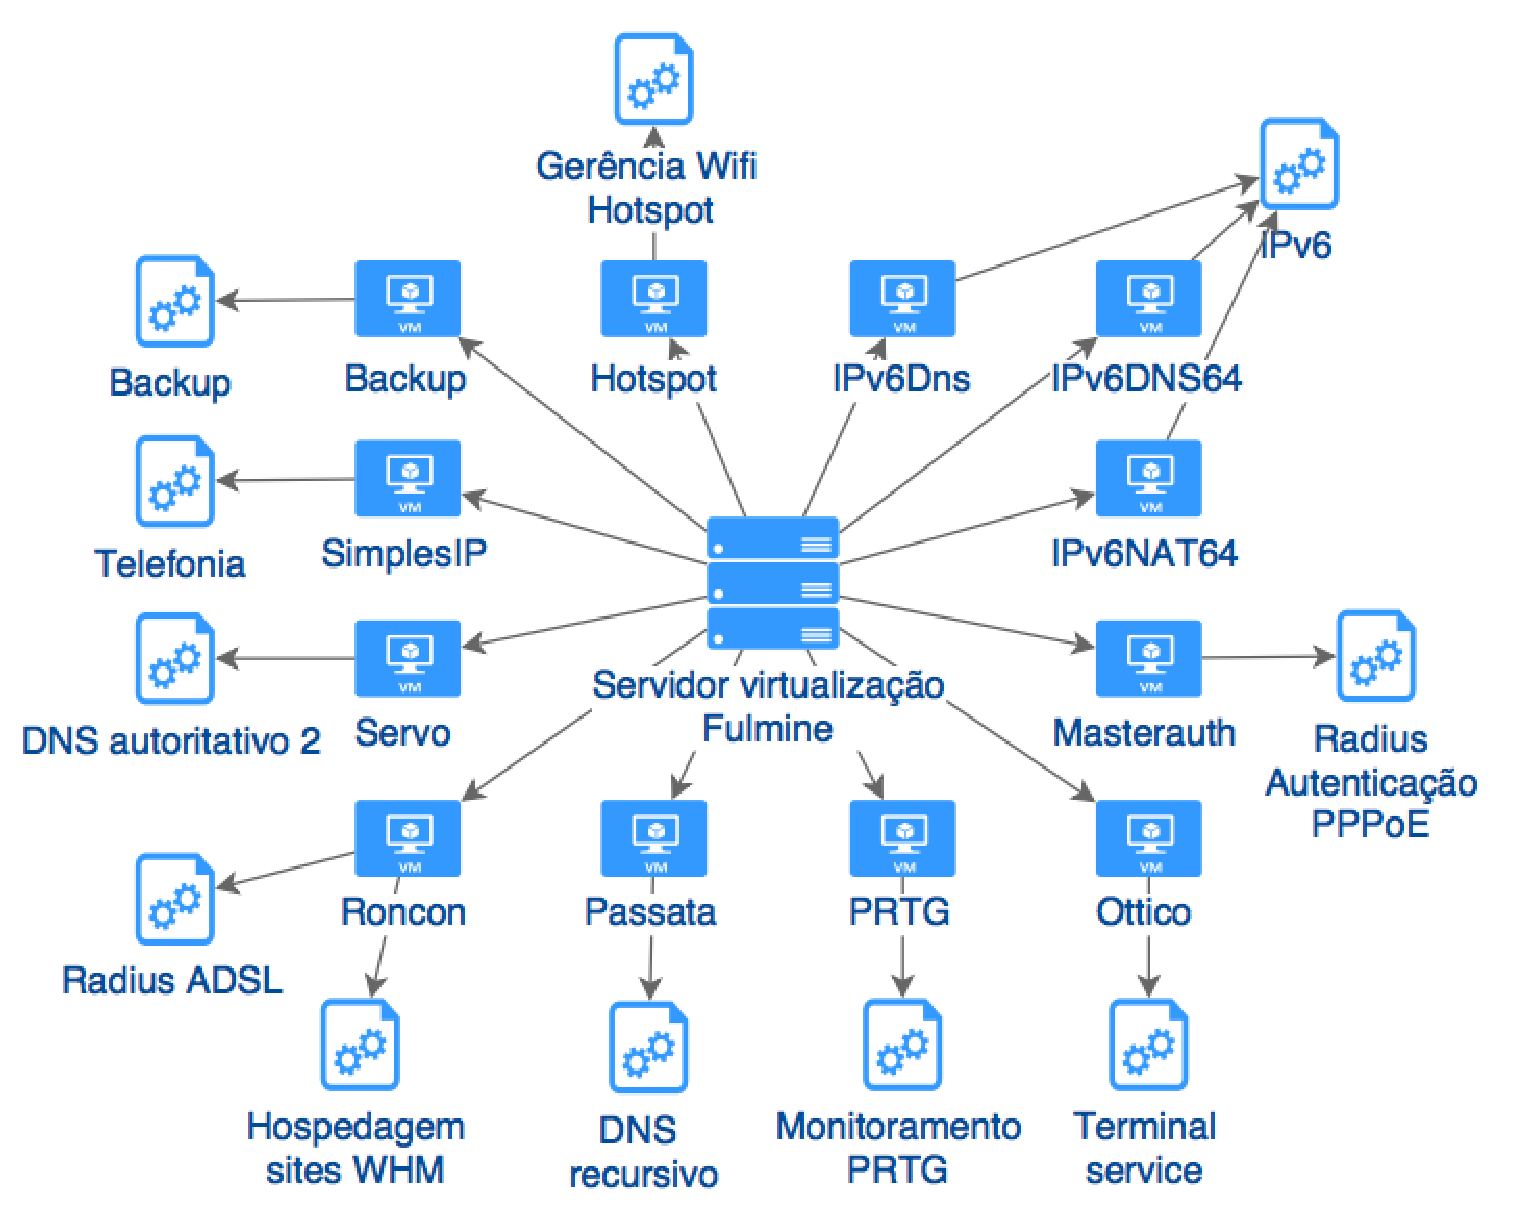
\includegraphics[width=420px]{img/serv_fulmine.eps}
 \caption{Servidor de virtualização Fulmine.}
 \label{fig:serv_fulmine}
\end{figure}

O servidor chamado Piova executa oito \ac{VM}s (Figura \ref{fig:serv_piova}), que fornecem os seguintes serviços:
\begin{itemize}
 \item \textit{ASP}: esse servidor possui 1 \textit{core} para processamento, 1 GB de memória e 50 GB de disco. O servidor possui o sistema 
 operacional \textit{Windows 2008 Server R2}. Esse servidor provê acesso a sites \textit{web} desenvolvidos com a linguagem \ac{ASP}, através do
 \textit{software} \textit{\ac{IIS} 7.5}. Sendo que possui aproximadamente dez sites hospedados;
 
 \item \textit{CactiBackbone}: esse servidor possui 1 \textit{core} para processamento, 1 GB de memória e 20 GB de disco. Ele é um servidor
 de monitoramento da rede do provedor. Esse utiliza a distribuição \textit{CentOS 6.3} e executa a aplicação \textit{Cacti 0.8.8a}. 
 Essa aplicação monitora atualmente uma parte da rede \textit{backbone} do provedor;
 
 \item \textit{Dio}: esse servidor possui 1 \textit{core} para processamento, 1 GB de memória e 17,8 GB de disco. O servidor possui o sistema 
 operacional \textit{Ubuntu 6.06 \ac{LTS}}. Esse servidor fornece serviço de hospedagens de sites desenvolvidos com a linguagem \ac{PHP} 
 versão 4.4.2, sendo que esses sites são mantidos devido a incompatibilidade com a versão 5. O número de sites é baixo, aproximadamente 10 sites;
 
 \item \textit{FateFurbo}: sua configuração é 2 \textit{cores} para processamento, 4 GB de memória e 80 GB de disco. O sistema operacional é o 
 \textit{Ubuntu 14.04 \ac{LTS}} \cite{ubuntu}. Ele possui um \textit{software} proprietário que faz a gerência de uma parte da fibra óptica do provedor;
 
 \item \textit{FiberHome}: sua configuração é 2 \textit{cores} para processamento, 2 GB de memória e 60 GB de disco. O sistema operacional é o 
 \textit{Windows XP}. Ele possui um \textit{software} para gerência da fibra óptica do provedor;
 
 \item \textit{Passata2}: esse servidor possui 1 \textit{core} para processamento, 2 GB de memória e 20 GB de disco. Esse servidor possui o 
 sistema operacional \textit{Ubuntu 14.04 \ac{LTS}} \cite{ubuntu}. Ele fornece o serviço de \ac{DNS} recursivo, através do \textit{software} 
 \textit{Bind 9.9.5}, e é o servidor secundário do provedor. A quantidade de requisições é ?? (Figura GRAFICO??);
 
 \item \textit{Postfix}: sua configuração é 1 \textit{core} para processamento, 768 MB de memória e 50 GB de disco. Esse servidor possui o 
 sistema operacional \textit{Ubuntu 14.04 \ac{LTS}} \cite{ubuntu}. Esse servidor faz o envio de e-mails, através do \textit{software} \textit{Postfix 2.11}.
 Os e-mails enviados por ele tem origem em uma ferramenta desenvolvida pela empresa, que é uma ferramenta de e-mail marketing, ou seja, 
 faz o envio de e-mails em massa para divulgação de informações ou produtos;
 
 \item \textit{Servo6}: sua configuração é 1 \textit{core} para processamento, 1,5 GB de memória e 30 GB de disco. Esse servidor possui o 
 sistema operacional \textit{CentOS 6.8}. Esse servidor fornece, através do \textit{software} \textit{Bind 9.8.2}, o serviço de \ac{DNS} 
 autoritativo e é o servidor \ac{DNS} terciário dos domínios hospedados pela empresa;
\end{itemize}

\begin{figure}[h!]
 \centering
 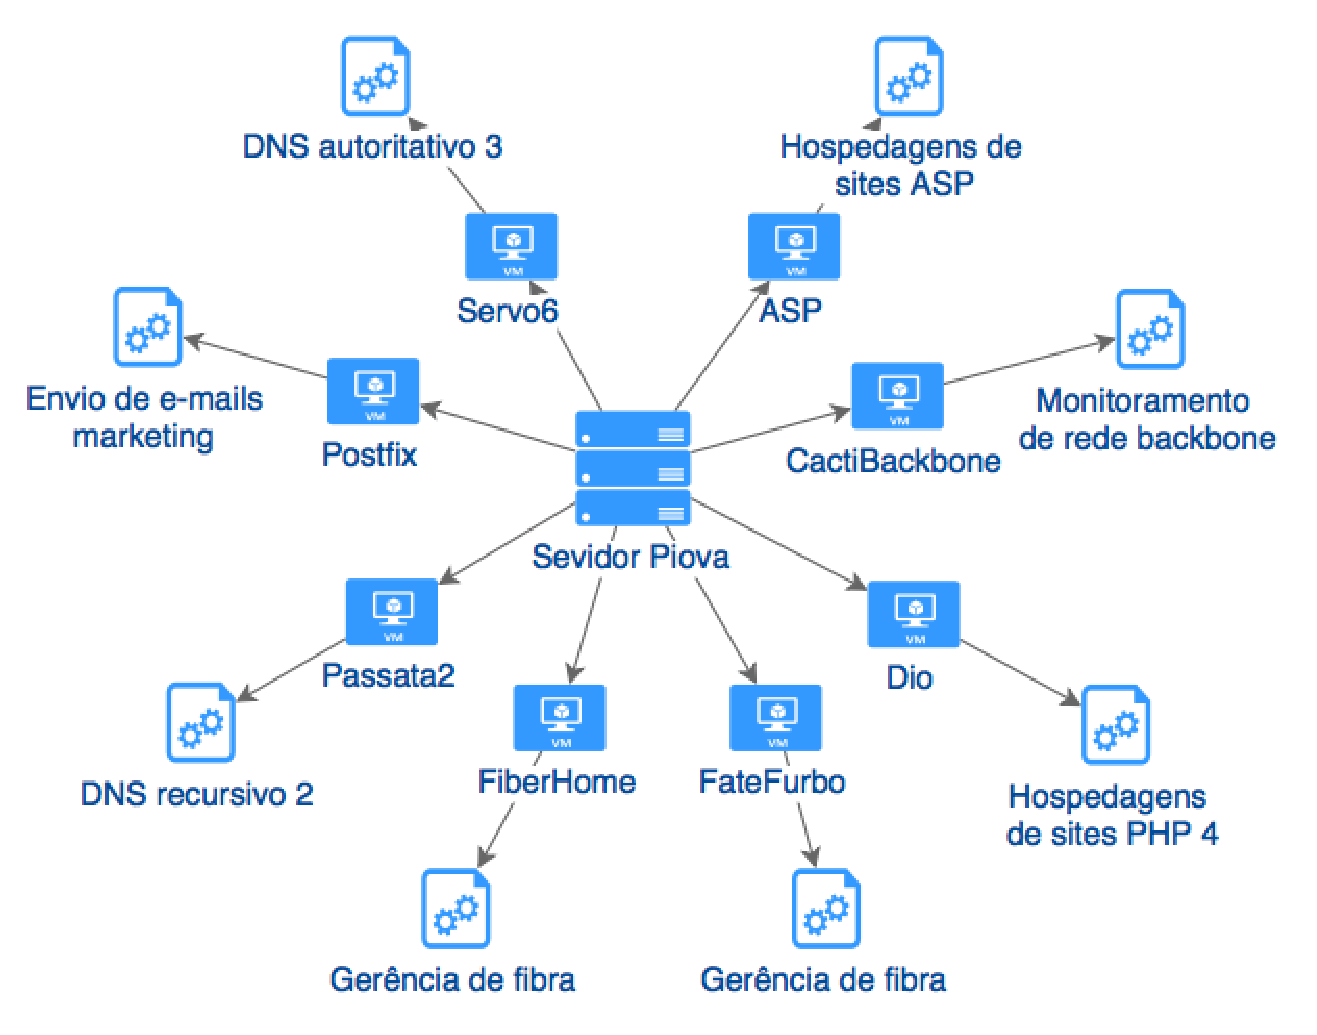
\includegraphics[width=430px]{img/serv_piova.eps}
 \caption{Servidor de virtualização Piova.}
 \label{fig:serv_piova}
\end{figure}

O servidor chamado Raggio executa doze \ac{VM}s (Figura \ref{fig:serv_raggio}), que fornecem os serviços de virtualização para algumas empresas. Sendo que as máquinas virtuais
são instaladas com o sistema operacional da preferência do cliente, e são disponibilizadas através de um acesso remoto, como por exemplo através
de \ac{SSH}.

\begin{figure}[h!]
 \centering
 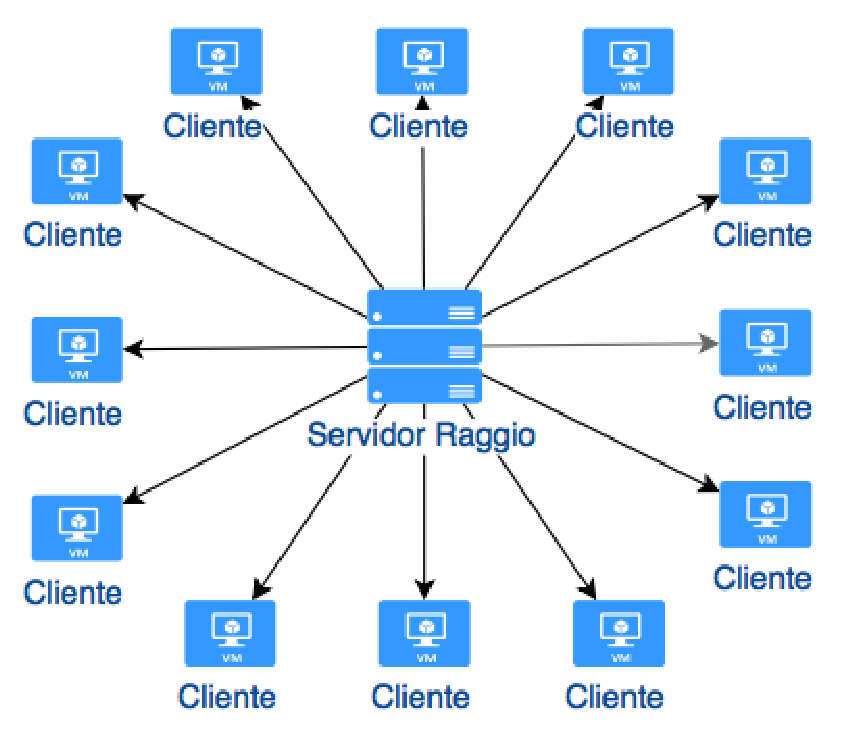
\includegraphics[width=300px]{img/serv_raggio.eps}
 \caption{Servidor de virtualização Raggio.}
 \label{fig:serv_raggio}
\end{figure}

O servidor chamado Tempesta executa uma \ac{VM} (Figura \ref{fig:serv_tempesta}), que fornecem os seguintes serviços:
\begin{itemize}
  \item \textit{Merak}: esse servidor virtual fornece serviço de e-mail. Ele possui uma configuração de 6 \textit{cores} para processamento, 
 10 GB de memória e 1000 GB de disco. O servidor possui o sistema operacional \textit{Windows 2008 Server R2} e executa o \textit{software} 
 \textit{Icewarp Server 10.4.4}. Essa aplicação fornece os serviços de envios de e-mails (\ac{SMTP}), recebimentos de e-mails (\ac{POP} e 
 \ac{IMAP}), Webmail (\ac{PHP}) e Anti-spam;
 %Possui ?? contas sendo que possui uma média de ?? usuários simultâneos...
 %Grande parte das contas estão ociosas pois são oferecidas juntamente com a internet vendida pelo provedor.

\end{itemize}

\begin{figure}[h!]
 \centering
 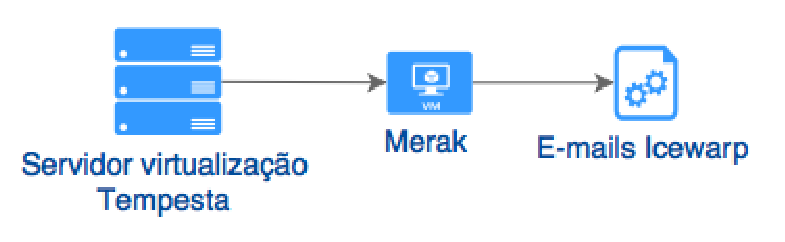
\includegraphics[width=260px]{img/serv_tempesta.eps}
 \caption{Servidor de virtualização Tempesta.}
 \label{fig:serv_tempesta}
\end{figure}

O servidor chamado Tuono executa oito \ac{VM}s (Figura \ref{fig:serv_tuono}), que fornecem os seguintes serviços:
\begin{itemize}
 \item \textit{Ledriovardar}: esse servidor possui 2 \textit{cores} para processamento, 2 GB de memória e 80 GB de disco. O servidor possui 
 o sistema operacional \textit{Windows 2008 Server R2}. Ele possui o serviço de \textit{terminal service} para suporte e gerência de fibra 
 óptica do provedor;
 
 \item \textit{Mondoperso}: sua configuração é 1 \textit{core} de processamento, 512 MB de memória e 8 GB de disco. Esse servidor possui o 
 sistema operacional \textit{Ubuntu 14.04 \ac{LTS}} \cite{ubuntu}. O servidor fornece \textit{streaming} de áudio para uma web rádio, esse serviço é feito
 através do \textit{software} livre \textit{Icecast 2.3.3};
 
 \item \textit{Monete}: sua configuração é 1 \textit{core} de processamento, 3 GB de memória e 50 GB de disco. Esse servidor possui o 
 sistema operacional \textit{Ubuntu 14.04 \ac{LTS}} \cite{ubuntu}. Esse é um servidor \textit{web} dedicado para o site do provedor, com configurações
 personalizadas. Para isso ele utiliza os \textit{softwares} \textit{Apache 2.4.7}, \textit{\ac{PHP} 5.5.9} (com \textit{PHP-FPM 5.59}), 
 \textit{MySQL 5.5.49};
 
 \item \textit{Ns}: esse servidor possui 1 \textit{core} para processamento, 2 GB de memória e 30 GB de disco. O servidor possui 
 o sistema operacional \textit{CentOS 6.8}. Esse servidor fornece, através do \textit{software} \textit{Bind 9.9.3}, o serviço de \ac{DNS} 
 autoritativo e é o servidor \ac{DNS} primário dos domínios hospedados pela empresa;
 
 \item \textit{Parla}: sua configuração é 1 \textit{core} de processamento, 1 GB de memória e 8 GB de disco. Ele possui o sistema
 operacional \textit{Ubuntu 14.04 \ac{LTS}} \cite{ubuntu}. Esse servidor provê um serviço de mensagens instantâneas, baseado no protocolo \ac{XMPP}, o que 
 facilita a comunicação entre funcionários da empresa e do provedor. O \textit{software} utilizado é o \textit{Ejabberd 2.1.11},
 que também é um \textit{software} livre;
 
 \item \textit{Rauco}: esse servidor possui 2 \textit{cores} para processamento, 6 GB de memória e 600 GB de disco. Ele possui o sistema
 operacional \textit{CentOS 6.8}. Esse servidor provê acesso a sites \textit{web} desenvolvidos com a linguagem \ac{PHP}. Nele está instalado o 
 \textit{software} \ac{WHM}, que faz a gerência dos serviços de hospedagens de sites e banco de dados. Além disso existe uma ferramenta que 
 faz parte do \ac{WHM} que é o \textit{cPanel}, sendo que ele fornece a gerência de cada hospedagem de site para seu respectivo desenvolvedor.
 Para fornecer essa hospedagem os seguintes \textit{softwares} estão instalados e configurados: \textit{Apache 2.4.18}, \textit{\ac{PHP} 5.6.21}, 
 \textit{MySQL 5.5.49} e \textit{PostgreSQL 8.4.20};
 
 \item \textit{Soldi}: sua configuração é 4 \textit{cores} de processamento, 4 GB de memória e 40 GB de disco. Esse servidor possui o 
 sistema operacional \textit{Ubuntu 14.04 \ac{LTS}} \cite{ubuntu}. Esse é um servidor \textit{web} exclusivo para \textit{softwares} de gestão desenvolvidos
 pela empresa. Os seguintes \textit{softwares} são utilizados: \textit{Apache 2.4.7}, \textit{\ac{PHP} 5.5.9} (com \textit{PHP-FPM 5.59}), 
 \textit{MySQL 5.5.49};
 
 \item \textit{Trapel}: sua configuração é 1 \textit{core} de processamento, 768 MB de memória e 8 GB de disco. Esse servidor possui o 
 sistema operacional \textit{Ubuntu 14.04 \ac{LTS}} \cite{ubuntu}. Ele fornece um serviço de teste de velocidade da conexão de internet, os 
 usuários do provedor utilizam esse serviço para testar a velocidade da sua internet. Para isso ele executa as aplicações \textit{Apache 2.4.7} e
 \textit{\ac{PHP} 5.5.9}, e um \textit{software} desenvolvido pelo \textit{SpeedTest} \cite{speedtest};
\end{itemize}

\begin{figure}[h!]
 \centering
 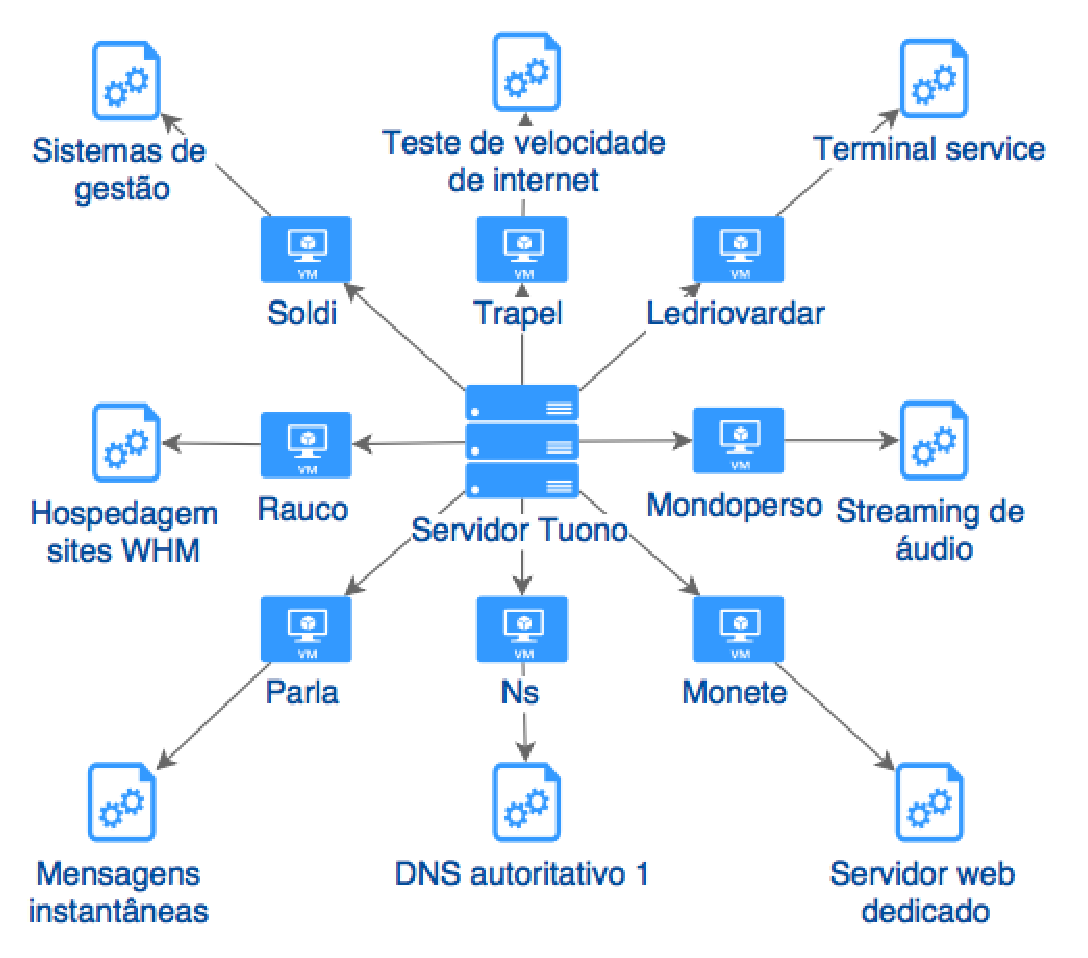
\includegraphics[width=360px]{img/serv_tuono.eps}
 \caption{Servidor de virtualização Tuono.}
 \label{fig:serv_tuono}
\end{figure}

\subsection{Servidor Venti}
\label{section:serv_venti}

O servidor chamado Venti executa cinco \ac{VM}s (Figura \ref{fig:serv_venti}), que fornecem os seguintes serviços:
\begin{itemize}
 \item \textit{Backup}: sua configuração é 1 \textit{core} para processamento, 1 GB de memória e 15 GB de disco. Esse servidor possui o 
 sistema operacional \textit{Ubuntu 14.04 \ac{LTS}} \cite{ubuntu}. Nele é executado o serviço de \textit{backup} dos equipamentos do provedor, para isso 
 é utilizado \textit{scripts} que buscam e copiam os dados através do protoccolo \ac{FTP};
 
 \item \textit{Esibire}: sua configuração é 1 \textit{core} para processamento, 1 GB de memória e 50 GB de disco. Esse servidor possui o 
 sistema operacional \textit{Ubuntu 14.04 \ac{LTS}} \cite{ubuntu}. Esse servidor faz a hospedagem de vídeos e a reprodução de \textit{streaming} utilizando
 \ac{FTP} e um servidor \textit{web} \textit{Apache 2.4.7};
 
 \item \textit{Miatanto}: sua configuração é 1 \textit{core} de processamento, 1 GB de memória e 8 GB de disco. Esse servidor possui o 
 sistema operacional \textit{Ubuntu 14.04 \ac{LTS}} \cite{ubuntu}. O servidor fornece \textit{streaming} de áudio para uma web rádio, esse serviço é feito
 através do \textit{software} livre \textit{Icecast 2.3.3};
 
 \item \textit{Pomodoro}: sua configuração é 1 \textit{core} de processamento, 2 GB de memória e 28 GB de disco. Esse servidor possui o 
 sistema operacional \textit{Ubuntu 14.04 \ac{LTS}} \cite{ubuntu}. Esse servidor faz a documentação dos equipamentos do provedor, utilizando a aplicação
 open source? \textit{Sakai 2.9};
 
 \item \textit{Quebei}: sua configuração é 1 \textit{core} de processamento, 3 GB de memória e 140 GB de disco. Esse servidor possui o 
 sistema operacional \textit{Ubuntu 14.04 \ac{LTS}} \cite{ubuntu}. Sua função é gerenciar o \textit{backup} dos outros servidores, para isso ele utiliza a 
 ferramenta \textit{Bacula 5.2.6} (pacote \textit{bacula-director-common 5.2.6}). Além disso, esse servidor possui o sistema gerenciador de 
 banco de dados \textit{MySQL 5.5.49} instalado, que esta configurado como \textit{master-slave}, sendo que esse servidor é o \textit{slave} e 
 o servidor \textit{Dati} é o \textit{master};
\end{itemize}

\begin{figure}[h!]
 \centering
 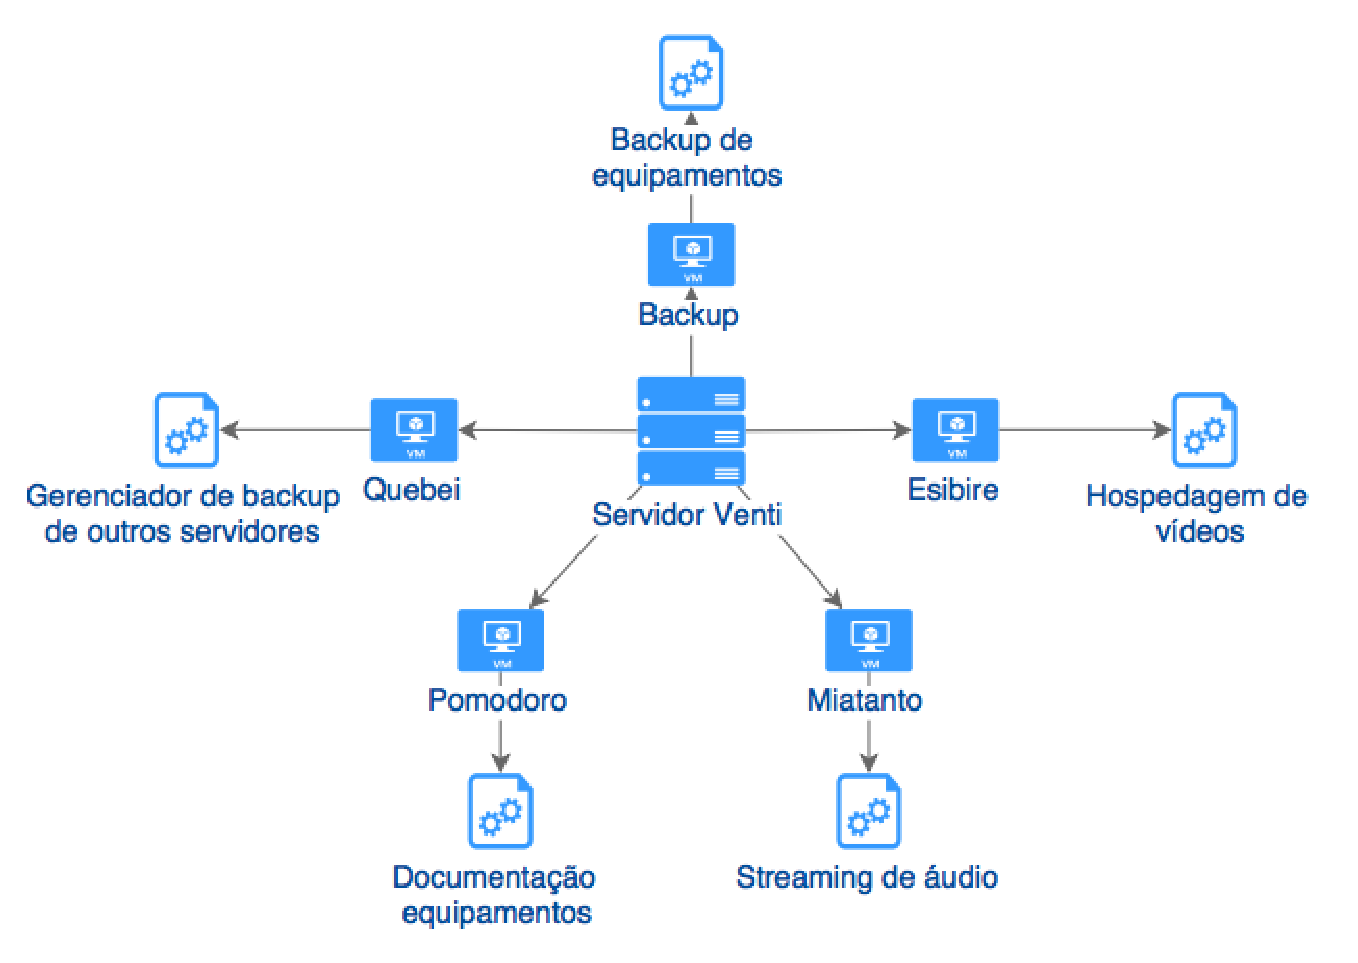
\includegraphics[width=430px]{img/serv_venti.eps}
 \caption{Servidor de virtualização Venti.}
 \label{fig:serv_venti}
\end{figure}

-graficos cpu memoria disco cada servidor de virtualizacao?? colocar aqui ou na implementacao??

-citar ferramentas monitoramento, gerenciamento, update e backup??

\section{Serviços críticos}
\label{section:servcrit}

Na seção anterior foram detalhados todos os serviços que estão atualmente disponíveis na empresa, com isso nesta seção será feito a 
idenficação dos serviços mais críticos para a empresa. Sendo assim os seguintes critérios serão 
utilizados para selecionar esses serviços críticos, para possibilitar a implementação do ambiente de alta disponibilidade: 
\begin{itemize}
 \item A quantidade de clientes ou funcionários que utilizam o serviço: esse é o item mais relevante, pois impacta diretamente no faturamento
 da empresa. Por exemplo, se um cliente ficar sem acesso à internet, a sua mensalidade pode ser reduzida de acordo com o tempo que ele ficou
 sem acesso; 
 \item O número de requisições em um determinado tempo: esse número é importante, devido ao fato de indicar ações dos usuários. Sabe-se que
 quanto mais ações, mais usuários dependem do serviço. São exemplos dessa medida: quantidade de acessos por minuto em um servidor de hospedagens 
 de sites, ou quantidade de requisições \ac{DNS} em um servidor recursivo;
 \item O volume de objetos do serviço: essa medida demonstra a abrangência do serviço, ou seja, qual a demanda que o serviço pode atingir.
 Por exemplo, a quantidade de equipamentos monitorados por um servidor de monitoramento.
\end{itemize}

Deste modo, pode-se afirmar que esses critérios são importantes, pois caso os serviços relacionados a eles ficarem indisponíveis causarão 
um prejuízo financeiro para a empresa. 

Os serviços mais críticos estão listados a seguir e ordenados de acordo com sua relevância:
\begin{itemize}
 \item \ac{DNS} recursivo primário: esse serviço foi classificado como mais importante pois possui um impacto direto nos clientes do provedor, e 
 é o único serviço que todos os clientes utilizam, que totalizam aproximadamente 9000 clientes. Sendo um provedor de internet, sua prioridade é 
 fornecer uma navegação de qualidade aos seus clientes, sendo assim o \ac{DNS} é fundamental para essa navegação. Outro importante critério é o 
 número de requisições por segundo (Figura GRAFICO??), que é o maior entre todos os outros serviços;
 
 \item \textit{Radius}: esse serviço também é importante para navegação dos clientes do provedor, pois, como visto anteriormente, ele faz a
 autenticação dos clientes de acesso a internet de todo o provedor, que chega aproximadamente a 9000 clientes. Caso esse serviço fique 
 indisponível os clientes não conseguirão estabelecer conexão para navegar, sabendo que atualmente esse serviço recebe x?? requisições de
 autenticação por segundo (Figura GRAFICO FREERADIUS??). Além disso, esse serviço armazena dados de clientes como: o endereço de \ac{IP} de cada 
 cliente utilizado em um determinado período, o tráfego de dados da conexão, o tempo da conexão de cada cliente, entre outros. 
 Essas operações resultam em um número de requisições por segundo, que esta detalhado na Figura GRAFICO??;
 
 \item Sistemas: esse serviço não tem um grande impacto direto para os clientes, porém tem um grande impacto para os funcionários da empresa e 
 do provedor. Totalizando x?? funcionários, caso houver uma indisponibilidade dos sistemas a maior parte desses funcionários ficarão 
 impossibilitados de trabalhar (aproximadamente x?? funcionários simultâneos de acordo com a Figura GRAFICO??), isso poderia gerar um prejuizo 
 elevado para a empresa e o provedor. Sendo que o sistema do provedor é responsável pela maior parte das operações do provedor, 
 como por exemplo, emissão de boletos e envio para clientes, atendimento de clientes, comunicação interna da empresa, vendas, 
 ativações de novos clientes, entre outros;
 
 \item Telefonia: esse serviço tem relevância para a empresa e para o provedor, pois permite a comunicação entre clientes e funcionários, 
 e também entre funcionários e outros funcionários, sendo essencial para qualquer empresa. Sabendo que possui uma média de x?? ligações por xx
 (Figura GRAFICO??), sendo que essas ligações são utilizadas por todos o setores do provedor e também da empresa. Exemplos práticos são: 
 atendimento a clientes para suporte técnico, comunicação interna entre funcionários, comunicação com técnicos externos, cobranças a clientes 
 inadimplentes, vendas, entre outros. Levando isso em consideração, se esse serviço ficar indisponível irá gerar prejuízos para a empresa.
\end{itemize}

Tendo esses serviços, pode-se identificar quais máquinas virtuais serão incluídas no ambiente de alta disponibilidade, que são:
\begin{itemize}
 \item \textit{Passata}
 \item \textit{Speedauth}
 \item \textit{Masterauth}
 \item \textit{Soldi}
 \item \textit{SimplesIP}
\end{itemize}

Sendo assim, os recursos das máquinas virtuais, citadas anteriormente, somados são 11 \textit{cores} de processamento, 12 GB de memória e 156 GB de disco.

-Exibir disponibilidade média atual dos serviços, com gráficos??

\section{Considerações finais}

Neste capítulo foi apresentado a empresa e feito uma análise de seus serviços. Com isso no próximo capítulo será desenvolvido uma proposta 
para implementação de um ambiente de alta disponibilidade nos servidores de virtualização da empresa, além de identificar as ferramentas
que serão utilizadas para essa implementação.


%Esboço: \\
%-DNS (impacto direto para clientes e rede interna): \\
%requisicoes por segundo\\
%numero de usuarios\\
%-Radius (impacto direto para clientes): \\
%numero de usuarios autentidados em x tempo\\
%quantidade de dados armazenados no db em x tempo, tráfego utilizado, tempo conexao\\
%numero de usuarios\\
%-Sistemas (impacto indireto para clientes): \\
%gasto com funcionarios ociosos\\
%quantidade de atendimento a clientes\\
%numero de cobrancas enviadas para clientes efetuar pagamento\\
%comunicacao entre setores e funcionarios\\
%numero de usuarios\\
%-Telefonia (impacto indireto para clientes): \\
%quantidade de atendimento a clientes\\
%comunicacao entre setores e funcionarios\\
%ligacoes saintes, atendimento, cobranca, tecnicos instalacoes internet\\
%numero de usuarios\\

